\documentclass[xcolor=dvipsnames]{beamer} 
\usecolortheme[named=Blue]{structure} 
\usetheme[height=10.5mm]{Rochester} 
\setbeamertemplate{items}[ball] 
\setbeamertemplate{blocks}[rounded][shadow=true] 
\setbeamertemplate{navigation symbols}{} 
\usepackage{bm}
\usepackage{listings}
\usepackage{rotating}
\usepackage{graphicx}
\usepackage{multirow}
\usepackage{hyperref}
\usepackage{textcomp}
\usepackage{upquote}
\usepackage[absolute,overlay]{textpos}
\newenvironment{reference}[2]{%
  \begin{textblock*}{\textwidth}(#1,#2)
      \footnotesize\it\bgroup\color{red!50!black}}{\egroup\end{textblock*}}
%\graphicspath{ {/home/ben/PhD/Armidale_Updates/2014_03_14/Figures/} }
\begin{document}

%%% New plan for this module:
%%% we all use Git on the command line and view GitHub in our web browsers
%%% clone and commit via HTTPS
%%% Workflow plan:
%%%
%%% Create repo in web browser
%%% Authenticate on cmd line
%%% Clone
%%% Add files
%%% Edit
%%% git add
%%% git commit
%%% branch and revert to previous version with check out


%%% Getting on the command line in various OS's

%%% MS Windows -> Start Menue -> Powershell
%%% Mac OS -> Finder -> terminal
%%% GNU+Linux users -> application launcher (will vary depending on GUI) -> terminal 


\begin{frame} %1
% \frametitle{Addressing Common Challenges in Spatial Modeling of Ecologies and Environments}
\begin{center}
\textbf{\huge Version Control with Git}\\
\end{center}

\begin{figure}
%\includegraphics[width = 0.35\textwidth]{/home/ben/Intro_to_R/GitHub_Slides_Source/Images/GitHub-Mark-120px-plus.png}
\begin{columns}

\begin{column}{3.3cm}
\begin{center}
\begin{figure}

\includegraphics[width = 0.9\textwidth]{/home/ben/Intro_to_R/Introductory_Slides_Source/Images/R_logo.png}
\end{figure}
\end{center}
\end{column} 

\begin{column}{3.3cm}
\begin{center}
\begin{figure}

\includegraphics[width = 0.9\textwidth]{/home/ben/Intro_to_R/GitHub_Slides_Source/Images/Git-Icon-1788C.pdf}
\end{figure}
\end{center}
\end{column} 

\begin{column}{3.3cm}
\begin{center}
\begin{figure}

\includegraphics[width = 0.9\textwidth]{/home/ben/Intro_to_R/GitHub_Slides_Source/Images/GitHub-Mark_Big.pdf}
\end{figure}
\end{center}
\end{column} 

\end{columns}
\end{figure}

\small Ben R. Fitzpatrick\\
\tiny PhD Candidate, Statistical Science, Mathematical Sciences School, Queensland University of Technology
\newline
\begin{columns}
\begin{column}{3cm}
\tiny 0000-0003-1916-0939
\end{column}
\begin{column}{3cm}
\tiny github.com/brfitzpatrick/
\end{column}
\begin{column}{3cm}
\tiny @benrfitzpatrick
\end{column}
\end{columns}
\end{frame}


\begin{frame}
\frametitle{Version Control Software}
Have you ever put numbers or dates at the end of a file name to keep different versions of it? 
\begin{itemize} 
\item If yes then you have already used version control!
\newline
\newline
\end{itemize}

Have you ever used track changes and comments to take turns editing a  MS Word document with one or more others?
\begin{itemize}
\item If yes then you have collaboratively edited a file!
\newline
\newline
\end{itemize}

Version Control Software: 
\begin{itemize} 
\item formalizes these concepts
\item can do a lot of the organisational work for you
\item makes reverting to previous versions without losing work easy 
\end{itemize}
 
\end{frame}

\begin{frame}
\frametitle{Version Control when Working Alone}
\begin{block}{Version Control for Solo Authoring File}
\begin{itemize}
\item You essentially have a time stamped undo button which will allow you to go review or revert to previous versions of the file
\item you can even make multiple child versions fo the same file say for different audiences or to trial different orders and styles in which to write a report or program
\end{itemize}
\end{block}

\end{frame}


\begin{frame}
\frametitle{Version Control when Collaborating}
Greatly simplifies your life
Control over which changes different contributers make get added to the definitive version of a file
support for file to split into two child copies which can then be edited towards very different end points but still having the option to systematically recombine them at any stage

\end{frame}






\begin{frame}
\frametitle{Why Git?}

Git is free and open source
\newline
\newline
Git is available for most operating systems
\newline
\newline
Git is Distributed and Fast
\newline
\newline
Two major code hosting services (GitHub \& BitBucket) support version control with Git and both services have free account options

% \tiny $^1$ Google Code will close in 2016 as they have deemed it is no longer necessary given success of BitBucket and GitHub

\end{frame}



\begin{frame} 
\frametitle{Git is Distributed Version Control}
Every contributor has a copy of the entire database ( all revisions of all files)
two contributors can both work on the files in their copy of the database independently then their combined modifications can be merged systematically
\end{frame} 

\begin{frame}
\frametitle{Why Git on the Command Line?}
Makes discrete components of the workflow obvious this in turn will enable you to migrate easily to one of the many GUIs
\newline
\newline
The workflows we will practise today will work exactly the same way on MS Windows, MacOS and GNU+Linux
\newline
\newline
We have now been using a command line interface for 1.5 days to interact with the R program it's time to take it to the next level
\end{frame}

\begin{frame} 
\frametitle{Plan for this Module - Part 1}
\begin{block}{Solo Version Control}
\begin{itemize}
\item Set up Git on your laptops to communicate with the GitHub servers
\item Create a local `clone' of a remote repository
\item Make some changes to your local copy of the files
\item commit these changes to the git version control system
\item push these changes to your repository
\item make some more changes
\item revert to a previous version of the file
\end{itemize}
\end{block}
\end{frame}

\begin{frame} 
\frametitle{Plan for this Module - Part 2}

\begin{block}{Collaborating with Git \& GitHub}
\begin{itemize}
\item fork
\item branch 
\item edit
\item commit
\item pull request
\item merge
\end{itemize}
\end{block}

\end{frame}


\begin{frame}
\frametitle{Creating a Repository on the GitHub Servers}
\framesubtitle{Log into the GitHub Web Service}
\begin{center}
\begin{figure}
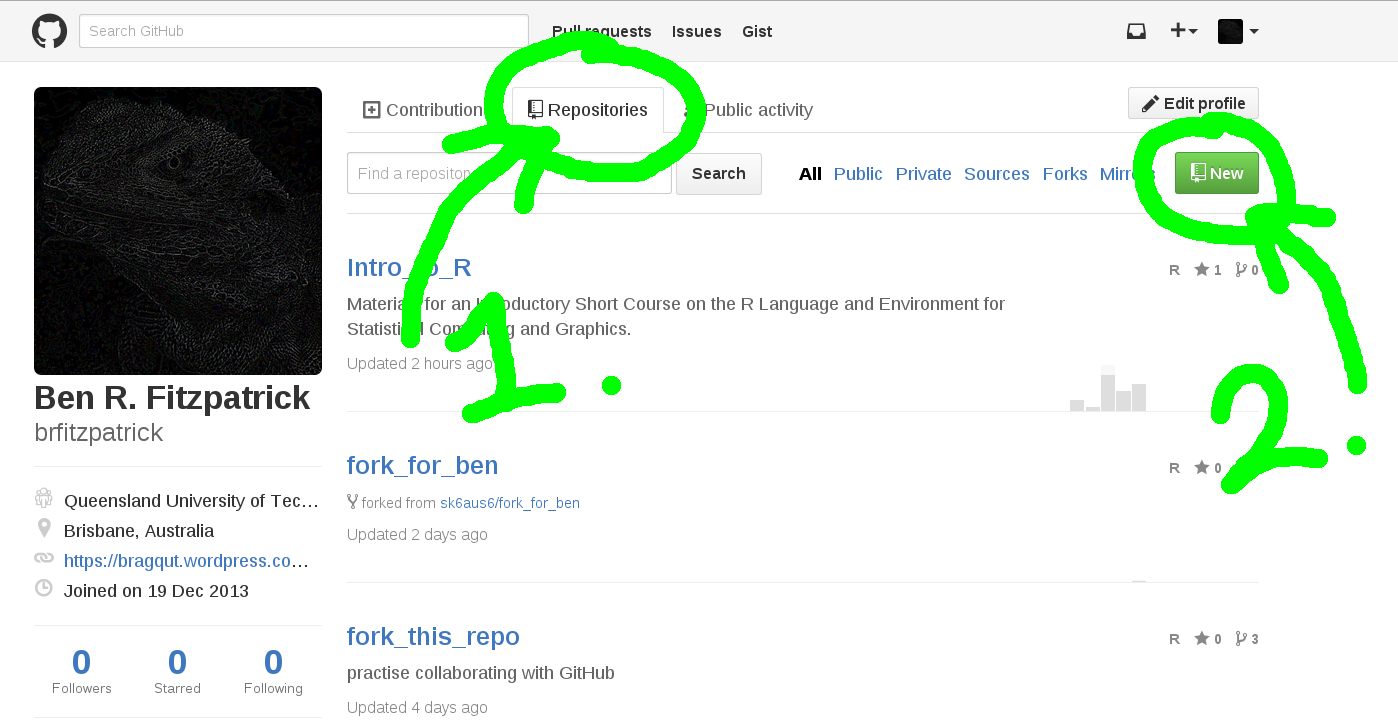
\includegraphics[width = \textwidth]{/home/ben/Intro_to_R/GitHub_Slides_Source/Images/New_Repo_1.png}
\end{figure}
\end{center}
\end{frame}

\begin{frame}
\frametitle{Creating a Repository on the GitHub Servers}
\framesubtitle{Complete the Details}
\begin{center}
\begin{figure}
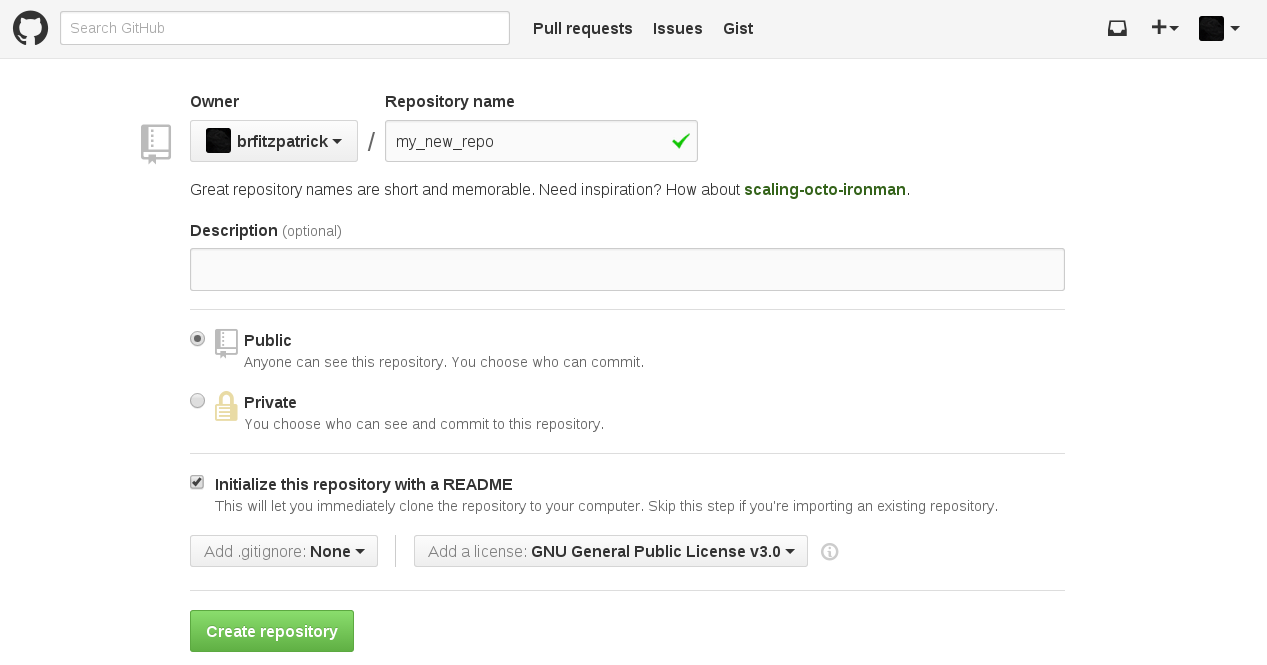
\includegraphics[width = \textwidth]{/home/ben/Intro_to_R/GitHub_Slides_Source/Images/New_Repo_2.png}
\end{figure}
\end{center}
\end{frame}

\begin{frame}
\frametitle{Creating a Repository on the GitHub Servers}
\framesubtitle{View your New Repository}
\begin{center}
\begin{figure}
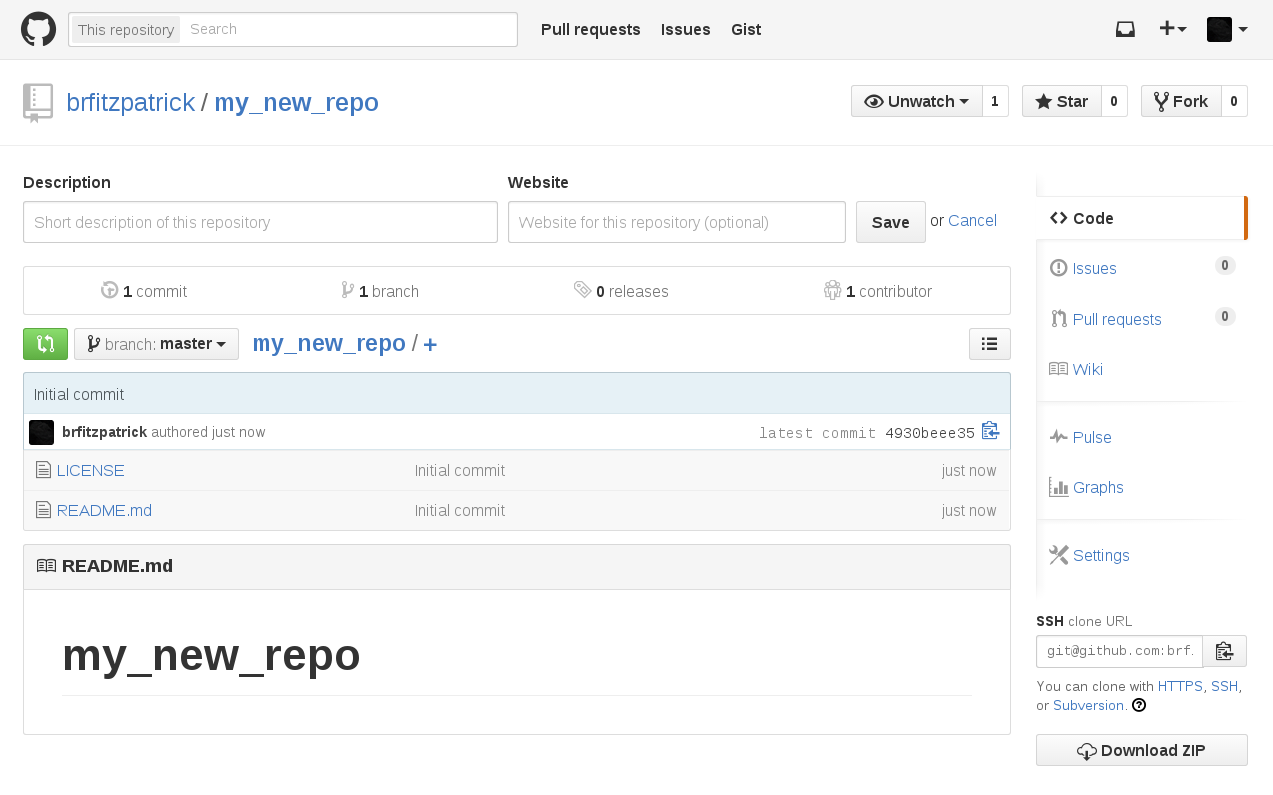
\includegraphics[width = \textwidth]{/home/ben/Intro_to_R/GitHub_Slides_Source/Images/New_Repo_3.png}
\end{figure}
\end{center}
\end{frame}

\begin{frame}
\frametitle{Cloning your new Repository to your Hard Drive}

First, create a folder on your Hard Drive in which to store your Git Repositories.  
\newline
\newline
We are now going to use the Git command line application to `clone' your new repository from the GitHub server to your hard drive.
\newline
\newline
Git is distributed version control so a Git `clone' is a complete copy of the entirity of the repository i.e.\begin{itemize}
\item all the files
\item the entire history of snapshots of files states created each time you committed to the respository
\newline \end{itemize}
Being a distributed version control system Git doesn't require you to be connected to the GitHub servers to work on your files and commit them to your branch of the repository.

\end{frame}

\begin{frame}
\frametitle{Git on the Command Line}
Accessing a command line interface in your OS of choice
\begin{columns}

\begin{column}{3.3cm}

\begin{center}
MS Windows\\
Open a `PowerShell'

\begin{figure}
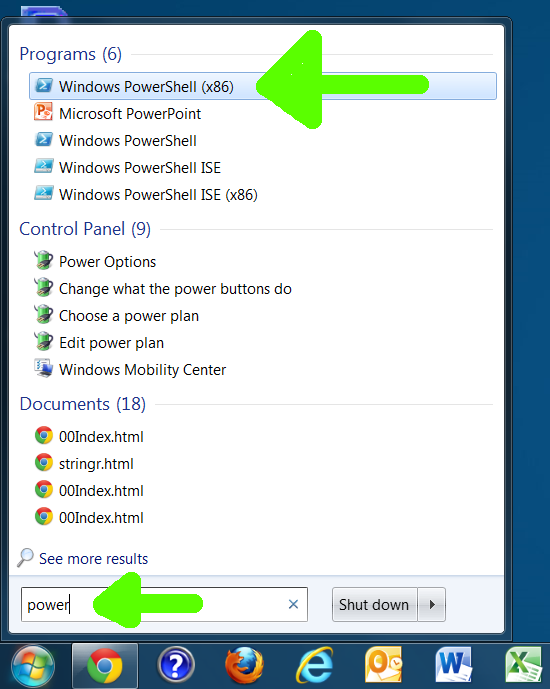
\includegraphics[width = \textwidth]{/home/ben/Intro_to_R/GitHub_Slides_Source/Images/Git_on_MS_Windows_Powershell/Powershell.png}
\end{figure}

\end{center}

\end{column} 

\begin{column}{3.3cm}
Mac OS X \& later\\
Open a `Terminal'
\begin{center}
\begin{figure}
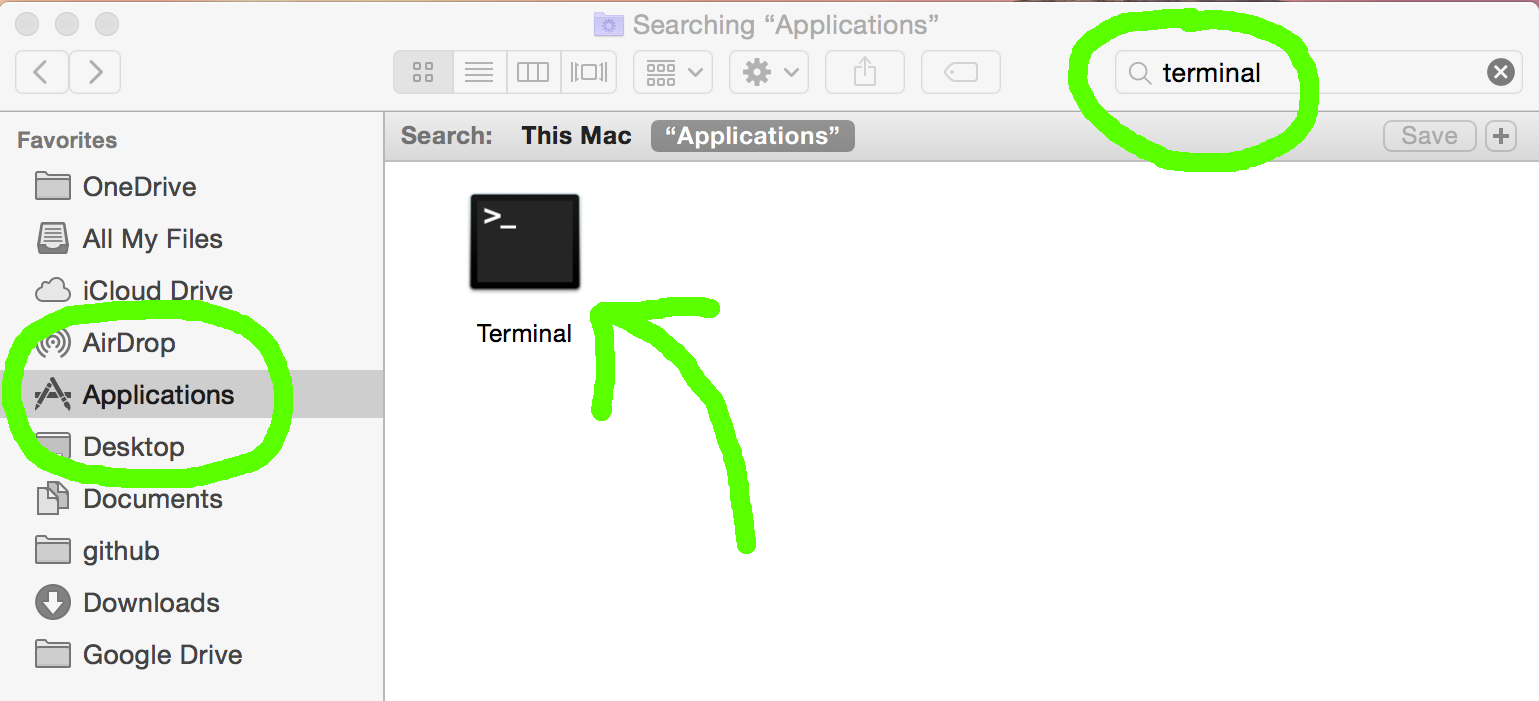
\includegraphics[width = \textwidth]{/home/ben/Intro_to_R/GitHub_Slides_Source/Images/Git_on_MacOS_Terminal/MacOS_Launch_Terminal_Annotated.png} %% insert MacOS Screenshot here
\end{figure}
\end{center}
\end{column} 

\begin{column}{3.3cm}

\begin{center}
GNU+Linux\\
Open a `Terminal'

\begin{figure}
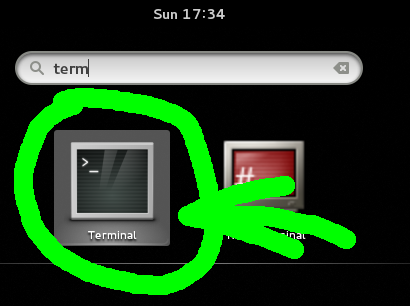
\includegraphics[width = \textwidth]{/home/ben/Intro_to_R/GitHub_Slides_Source/Images/Git_on_GNU_Linux_Terminal/Launch_Terminal.png}
\end{figure}

\end{center}

\end{column} 

\end{columns}
\end{frame}

\begin{frame}
\frametitle{Accessing a command line interface from MS Windows}
\framesubtitle{Open a `PowerShell'Powershell}
\begin{center}
\begin{figure}
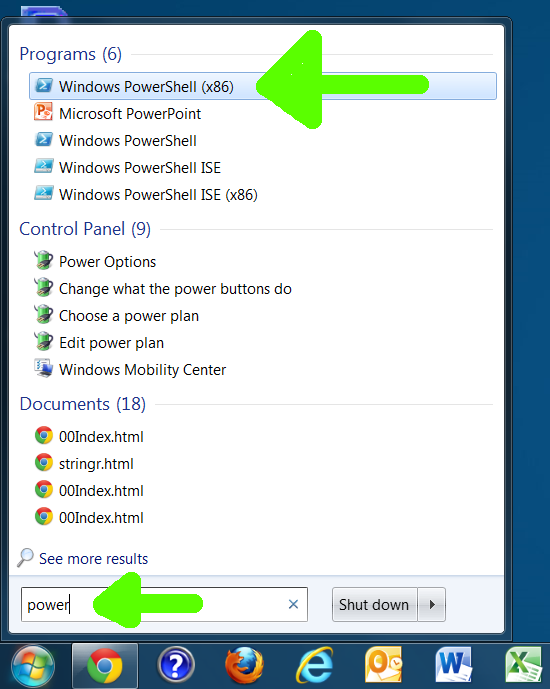
\includegraphics[height = 0.9\textheight]{/home/ben/Intro_to_R/GitHub_Slides_Source/Images/Git_on_MS_Windows_Powershell/Powershell.png}
\end{figure}
\end{center}
\end{frame}

\begin{frame}
\frametitle{Accessing a command line interface from MacOS}
\framesubtitle{Open a `Terminal'}
\begin{center}
\begin{figure}
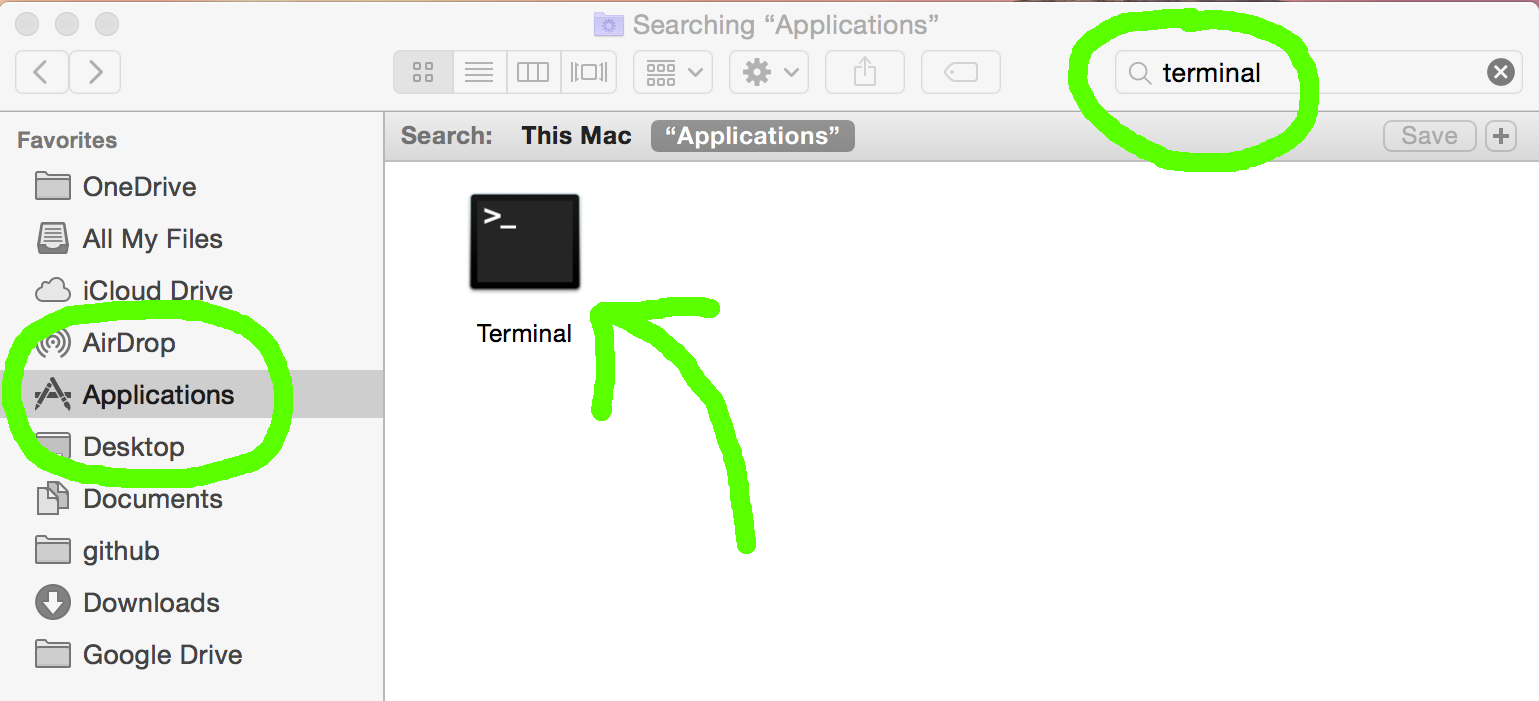
\includegraphics[width = \textwidth]{/home/ben/Intro_to_R/GitHub_Slides_Source/Images/Git_on_MacOS_Terminal/MacOS_Launch_Terminal_Annotated.png} 
\end{figure}
\end{center}
\end{frame}

\begin{frame}
\frametitle{Accessing a command line interface from GNU+Linux}
\framesubtitle{Open a `Terminal'}
\begin{center}
\begin{figure}
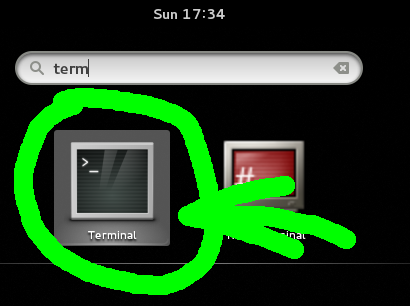
\includegraphics[height = 0.9\textheight]{/home/ben/Intro_to_R/GitHub_Slides_Source/Images/Git_on_GNU_Linux_Terminal/Launch_Terminal.png}
\end{figure}
\end{center}
\end{frame}

\begin{frame}[fragile]
\frametitle{Configuring Git for the first time}
\begin{block}{All Users}
\begin{lstlisting}
> git config --global user.name "Your Name"
> git config --global user.email you@mail.com
\end{lstlisting}
\end{block}
\end{frame}

\begin{frame}[fragile]
\frametitle{Configuring Git for the first time}
\framesubtitle{Choosing a Global Editor}
The global editor is used to write your commit messages.
\newline
\newline
Default is Vim but Vim is a little heavy on keyboard short cuts for some...
\newline
\newline
Many of the below can also function as an IDE for authoring R code if you prefer one of them to RStudio.
\newline
\newline
Other Options: \begin{itemize}
\item Notepad (available on all Windows PCs)
\item TextEdit (available on most Macs)
\item Atom: \url{https://atom.io/docs/v1.0.0/getting-started-installing-atom}
\item Sublime: \url{http://www.sublimetext.com/2}
\item TextMate: \url{http://macromates.com/download}
\item Emacs: \begin{verbatim} sudo apt-get install emacs \end{verbatim} 
\end{itemize}

\end{frame}

\begin{frame}[fragile]
\frametitle{Configuring Git for the first time}

\begin{block}{Set a Text Editor of your choice (you'll need it installed}
Use one of the below
\begin{lstlisting}
# Notepad:
> git config --global core.editor notepad.exe
# TextEdit:
> git config --global core.editor 'open -t -n -W'
# Atom:
> git config --global core.editor "atom --wait"
# Sublime:
> git config --global core.editor "subl -n -w"
# TextMate:
> git config --global core.editor "mate -w"
# Emacs:
> git config --global core.editor "emacs"
\end{lstlisting}
\end{block}

\end{frame}

\begin{frame}[fragile]
\frametitle{Cloning Your Repository from the GitHub Servers}

Set the working directory to the location on your hard drive to which you would like the repository cloned:

\begin{block}{Powershell Users}
\begin{lstlisting}
> C:
> cd C:\Users\username\Documents\GitHub_Repos\
> dir 
\end{lstlisting}
\end{block}

\begin{block}{Terminal Users}
\begin{lstlisting}
> cd /home/ben/Documents/GitHub_Repos
> ls 
\end{lstlisting}
\end{block}
\end{frame}

\begin{frame}
\frametitle{Copy HTTPS URL to use when cloning repository}
\begin{center}
\begin{figure}
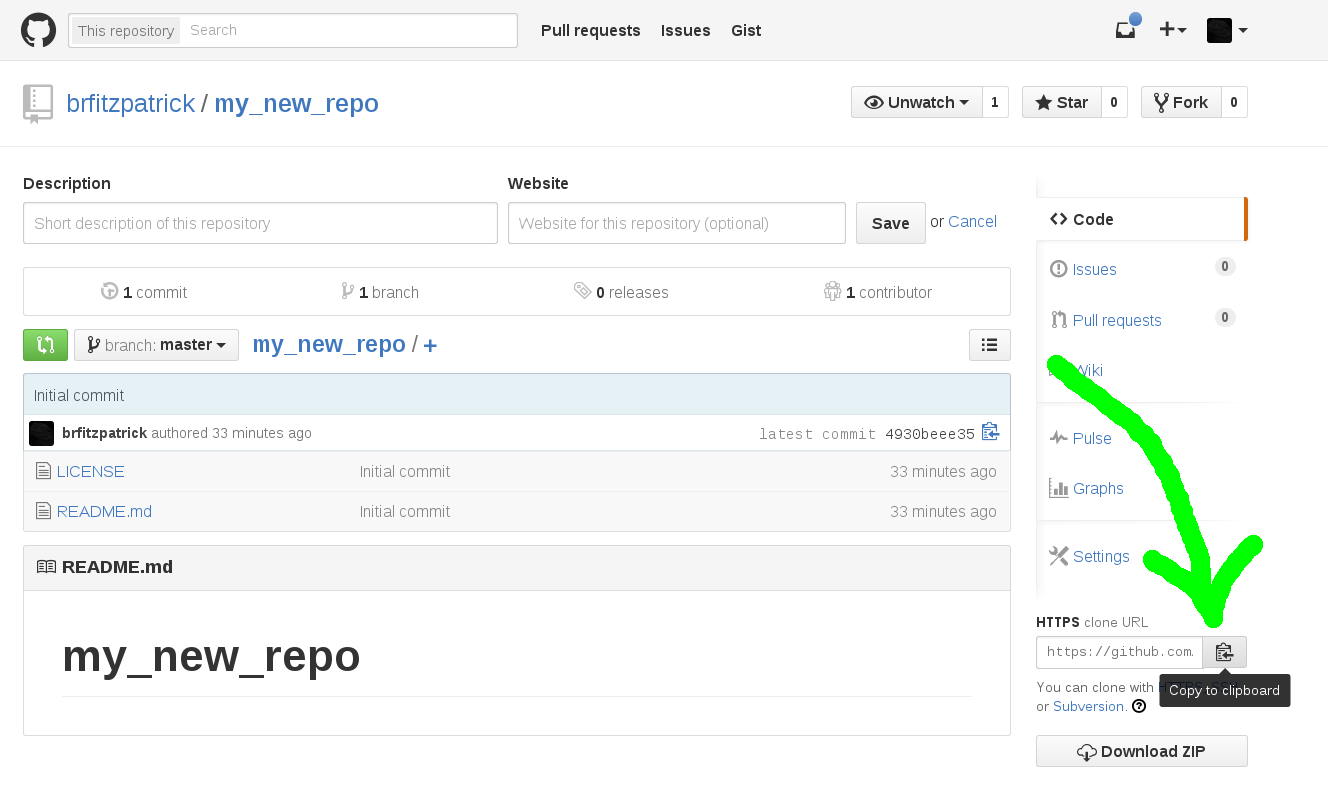
\includegraphics[width = \textwidth]{/home/ben/Intro_to_R/GitHub_Slides_Source/Images/Clone_Repo_1.png}
\end{figure}
\end{center}
\end{frame}

\begin{frame}[fragile]
\frametitle{Clone your Repository: GitHub Servers $\rightarrow$ your Hard Drive}
Use the HTTPS URL you copied earlier:\\
\begin{center}
\begin{figure}
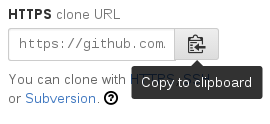
\includegraphics[width = 0.5\textwidth]{/home/ben/Intro_to_R/GitHub_Slides_Source/Images/HTTPS_Clone.png}
\end{figure}
\end{center}

\begin{block}{All Users}
\begin{lstlisting}
> git clone https://github.com/.../my_new_repo
  .git
> cd ./my_new_repo/
> ls
> git status
\end{lstlisting}
\end{block}
\end{frame}

\begin{frame} 
\frametitle{Git}
\framesubtitle{The Three States of Files in a Git Tracked Directory}
Files in a directory which you are version controlling with Git can exist in one of three states:
\begin{itemize}
\item \textbf{committed} data stored in the database for the associted repository
\item \textbf{modified} local copy of a file (in your working directory) is different to the most recent version of that file stored in the database for the associted repository i.e. you have changed something but not comitted the changes (yet)
\item \textbf{staged} the local copy of a file which you have modified is marked to be added to the database in the next commit snapshot you send to the database
\end{itemize}
\end{frame}

\begin{frame} 
\frametitle{Git}
\framesubtitle{Basic Git Workflow}
\begin{itemize}
\item you add files or modify existing files in your local copy of the repository
\item you stage these modified files ready to be committed to the database for the repository
\item you perform a commit which takes the files as they were when staged and stores a snapshot of them in the database for the repository
\end{itemize}
\end{frame}

\begin{frame}[fragile]
\frametitle{Git}
\framesubtitle{Adding New Files}
\begin{enumerate}
\item Open your favourite program for authoring R code (e.g. RStudio)
\item Create an new R script 
\item Save your R Script in the `clone' of your repository
\end{enumerate}

\end{frame}

\begin{frame}[fragile]
\frametitle{Git}
\framesubtitle{Adding New Files}

\begin{block}{}
\begin{lstlisting}
> git status
On branch master
Your branch is up-to-date with 'origin/master'.
Untracked files:
  (use "git add <file>..." to include in what 
will be committed)
\end{lstlisting}
\end{block}

We have to tell Git that we want it to track the changes we make to this new file

\end{frame}

\begin{frame}[fragile]
\frametitle{Git}
\framesubtitle{Adding New Files}

We have to tell Git that we want it to track the changes we make to this new file
\begin{block}{}
\begin{lstlisting}
> git add filename.R
> git status
On branch master
Your branch is up-to-date with 'origin/master'.
Changes to be committed:
  (use "git reset HEAD <file>..." to unstage)

	new file:   filename.R
\end{lstlisting}
\end{block}
We can still change our mind about adding the file to the repository at this stage quite easily.

\end{frame}

\begin{frame}[fragile]
\frametitle{Git}
\framesubtitle{Adding New Files}
Once you're ready to `commit' this change to the permanent record of changes in this repository we make a `commit'
\begin{block}{}
\begin{lstlisting}
> git commit
[master 311acfb] Initial Commit of some R code.
1 files changed, 0 insertions(+), 0 deletions
(-) create mode 100644 filename.R
\end{lstlisting}
\end{block}
You will be prompted to write a short description of the changes you are committing - these become invaluable as your project grows and if you are collaborating.
Once you've written a commit message, save it (and close the text editor if you used one).\\
You should see confirmation of the commit immediately below the git commit line.
\end{frame}

\begin{frame}[fragile]
\frametitle{Git}
Now that you've commited some changes to your local clone of the repository this local version will be ahead of the version on the GitHub Server
\begin{block}{}
\begin{lstlisting}
> git status
On branch master
Your branch is ahead of 'origin/master' by 1
commit.
 (use "git push" to publish your local commits)
\end{lstlisting}
\end{block}
Seeing as we are all currently connected to the internet, it's a good time to `push' these changes to GitHub server (`origin/master' in the default setup) to bring the remote copy of this repository up to date.
\end{frame}

\begin{frame}[fragile]
\begin{block}{pushing to the remote servers}
\begin{lstlisting}
> git push
Counting objects: 3, done.
Delta compression using up to 8 threads.
Compressing objects: 100\% (2/2), done.
Writing objects: 100\% (3/3), 353 bytes | 0 bytes/s, done.
Total 3 (delta 0), reused 0 (delta 0)
To git@github.com:brfitzpatrick/my_new_repo.git
   4930bee..99d61f1  master -> master
\end{lstlisting}
\end{block}
If you return to the page for your repository on the GitHub website and refresh the page you should see your most recent commit listed on the repository page.
\end{frame}

\begin{frame}[fragile]
\begin{block}{the whole process}
Furthermore, now that we have `commited' and `pushed' our most recent changes our local copy of the repository and the remote copy of the repository on the GitHub servers will be identical
\begin{lstlisting}
> git status
On branch master
Your branch is up-to-date with 'origin/master'.
nothing to commit, working directory clean
\end{lstlisting}
\end{block}
\end{frame}


%\begin{frame}[fragile]
%\begin{block}{the whole process}
%\begin{lstlisting}
%> git clone git@github.com:brfitzpatrick/my_new_repo.git
%Cloning into 'my_new_repo'...
%remote: Counting objects: 4, done.
%remote: Compressing objects: 100\% (3/3), done.
%remote: Total 4 (delta 0), reused 0 (delta 0), pack-reused 0
%Receiving objects: 100\% (4/4), 12.12 KiB | 0 bytes/s, done.
%Checking connectivity... done.
%> cd my_new_repo/
%> touch filename.R
%> emacs filename.R 
%> git add filename.R
%> git commit
%[master 99d61f1] My first commit of some R code.
% 1 file changed, 2 insertions(+)
% create mode 100644 filename.R
%> git push
%Counting objects: 3, done.
%Delta compression using up to 8 threads.
%Compressing objects: 100\% (2/2), done.
%Writing objects: 100\% (3/3), 353 bytes | 0 bytes/s, done.
%Total 3 (delta 0), reused 0 (delta 0)
%To git@github.com:brfitzpatrick/my_new_repo.git
%   4930bee..99d61f1  master -> master
%\end{lstlisting}
%\end{block}
%\end{frame}

\begin{frame} 
\frametitle{Undoing Things Safely}
\framesubtitle{Checking out Previous Commits to a New Branch}
To revert to a previous version of a file that you have `snapshot' of from a previous `commit'\\
Click on the file name on the GitHub website and click the `History' button:
\newline
\newline
Provided we have commited all changes to the file then it is safe to use the checkout command which will overwrite the file in the current local working directory with the file from the previous `commit'.
\newline
\newline
You can think of commits a bit like save points, if we have two we can move between them but if we load and old save without first making a current save we will loose the unsaveed changes
\end{frame}

\begin{frame} 
\frametitle{Git}
\framesubtitle{Undoing things}
choose a commit you'd like to go back to...copy the SHA
\newline
\newline
# List existing branches of current directory
git branch

# checkout a previous commit (SHA = 58...a44) 
\begin{verbatim}
> git checkout -b testing 589172506c13572be6cc052706ab4129de2c7a44
  Switched to a new branch 'testing'

> git branch
    master
  * testing

\end{verbatim}

Now if you open your .R file you'll see that you have a previous version of the file without the new changes

git branch

# make some changes on testing branch
# push those changes upsteam to server

git push --set-upstream origin testing

# check website - your repo should now have two branches

# Now to merge your changes from 'testing' back into 'master'

# to merge into a branch we must be on that branch:
git checkout master

# merge testing1 into current branch (master)
git merge testing1

Auto-merging Car_Bar_Charts.R
CONFLICT (content): Merge conflict in Car_Bar_Charts.R
Automatic merge failed; fix conflicts and then commit the result.

git mergetool

This message is displayed because 'merge.tool' is not configured.
See 'git mergetool --tool-help' or 'git help config' for more details.
'git mergetool' will now attempt to use one of the following tools:
meld opendiff kdiff3 tkdiff xxdiff tortoisemerge gvimdiff diffuse diffmerge ecmerge p4merge araxis bc3 codecompare emerge vimdiff
Merging:
Car_Bar_Charts.R

Normal merge conflict for 'Car_Bar_Charts.R':
  {local}: modified file
  {remote}: modified file
Hit return to start merge resolution tool (meld): 

## 

Now open you're R file to see the results of your merge







\newline
\newline
and open `filename.R' and our changes are gone
\newline
\newline
checkout the most recent commit to get them back
\newline
\newline
if you want to go back to a previous version of a file and try something new without overwriting your most recent versions you can `checkout' and old `commit' to a new `branch' of the repository

\end{frame}



\begin{frame}[fragile]
\frametitle{Git}
\framesubtitle{Undoing things}
One way to safely experiment with past versions of a file is to create a new `branch' in the repository in which to do so
\newline
\newline
branches are separate lines of development of the same files
\newline
\newline
let's make a new `testing3' branch checking out a previous version of the file filename.R\\
\begin{lstlisting}
> git checkout 99d61f19d85ae7aec691feb81ca8aef59f6a0719 -b testing3

> git push --set-upstream origin testing3
\end{lstlisting}
we can then move between branches with the checkout command
\begin{lstlisting}
> git checkout master

> git checkout testing3
\end{lstlisting}
\end{frame}

\begin{frame}[fragile]
  \frametitle{Merging Branches}
To merge the `master' and `testing3' branches
\begin{block}{}
\begin{lstlisting}
> git checkout master
> git merge testing3
\end{lstlisting}
\end{block}

if you get a merge conflict use a mergetool to resolve the conflict\\
(you should have one installed by default from when you installed Git)

\begin{block}{}
\begin{lstlisting}
> git mergetool
\end{lstlisting}
\end{block}
\end{frame}

%\begin{frame}[fragile]
%  \frametitle{Merging Branches}
%
%\begin{block}{once you have resolved the conflict}
% \begin{lstlisting}
%  > git add filename.R
%  > git commit
% \end{lstlisting}
% \end{block}

%\begin{block}{finally you can delete your testing branch if you're done with it}
% \begin{lstlisting}
%  > git branch -d testing3
% \end{lstlisting}
% \end{block}
%\end{frame}

%\begin{frame}
%\frametitle{Branching}
%
%%%'Branching means you diverge from the main line of development and continue to do work without messing with that main line.'

%Every project starts with the default `master' branch
%%%%you can then make a new branch e.g. a `testing' branch which will initially be the same as the `master' branch at the point in time at which you create it
%you switch to another branch by `checking out' that branch
%you can then commit changes to this branch without alterning the `master' branch i.e. you could develop some new feature without risking breaking the functionality of the master branch while you do so
%once your feel your work on the a branch is complete you can `merge' your `testing' branch with the `master' branch

%branching allows for collaboration, various contributors can all make their own branches of the repository then submit their changes to the repository owner for merging into the master branch - git provided powerful tools for managing these merges and resolving merge conflicts

%\end{frame}


\begin{frame}
\frametitle{Forking}
Fork a repository
Use the Sync button in Windows/MacOS client to get new changes from server (and submit any changes you have made)
\end{frame}

\begin{frame}
\frametitle{Create a Repository, Add Some Files}
\begin{itemize}
\item Log into your Github account
\item Click the Repositories Tab
\item Click the 'New' button (it's green)
\item name your repository
\item make it public (we can do a private one later)
\item intialize repository with a README
\item add a license GPL or MIT are easy FOSS licenses
\item clone the repository to your hard drive
\item add a file to your local clone of the repository
\item commit it to the repository
\item push your changes to the remote repository
\end{itemize}
\end{frame}

\begin{frame}
\frametitle{Fork a Friends Repository, Add Some Files}
\begin{itemize}
\item search for a friend's github repository
\item on their repository page click fork
\item clone your fork of their repository to your hard drive
\item edit one of their files
\item push your chages to their repo
\end{itemize}
\end{frame}

\begin{frame}
\frametitle{Accepting and rejecting Pull Requests}
\framesubtitle{Merging your friends' branches}
\end{frame}

\begin{frame}
\frametitle{Recommended Further Reading}
\framesubtitle{\url{http://git-scm.com/book/en/v2}}
\begin{center}
\begin{figure}

\includegraphics[height = 0.8\textheight]{/home/ben/Intro_to_R/GitHub_Slides_Source/Images/Git_Resources/ProGitCover.pdf}
\end{figure}
\cite{Chacon2014}
\end{center}

\end{frame}

\begin{frame}
\frametitle{Recommended Further Reading:}
\framesubtitle{\url{https://help.github.com/}}
%
\begin{center}
\begin{figure}
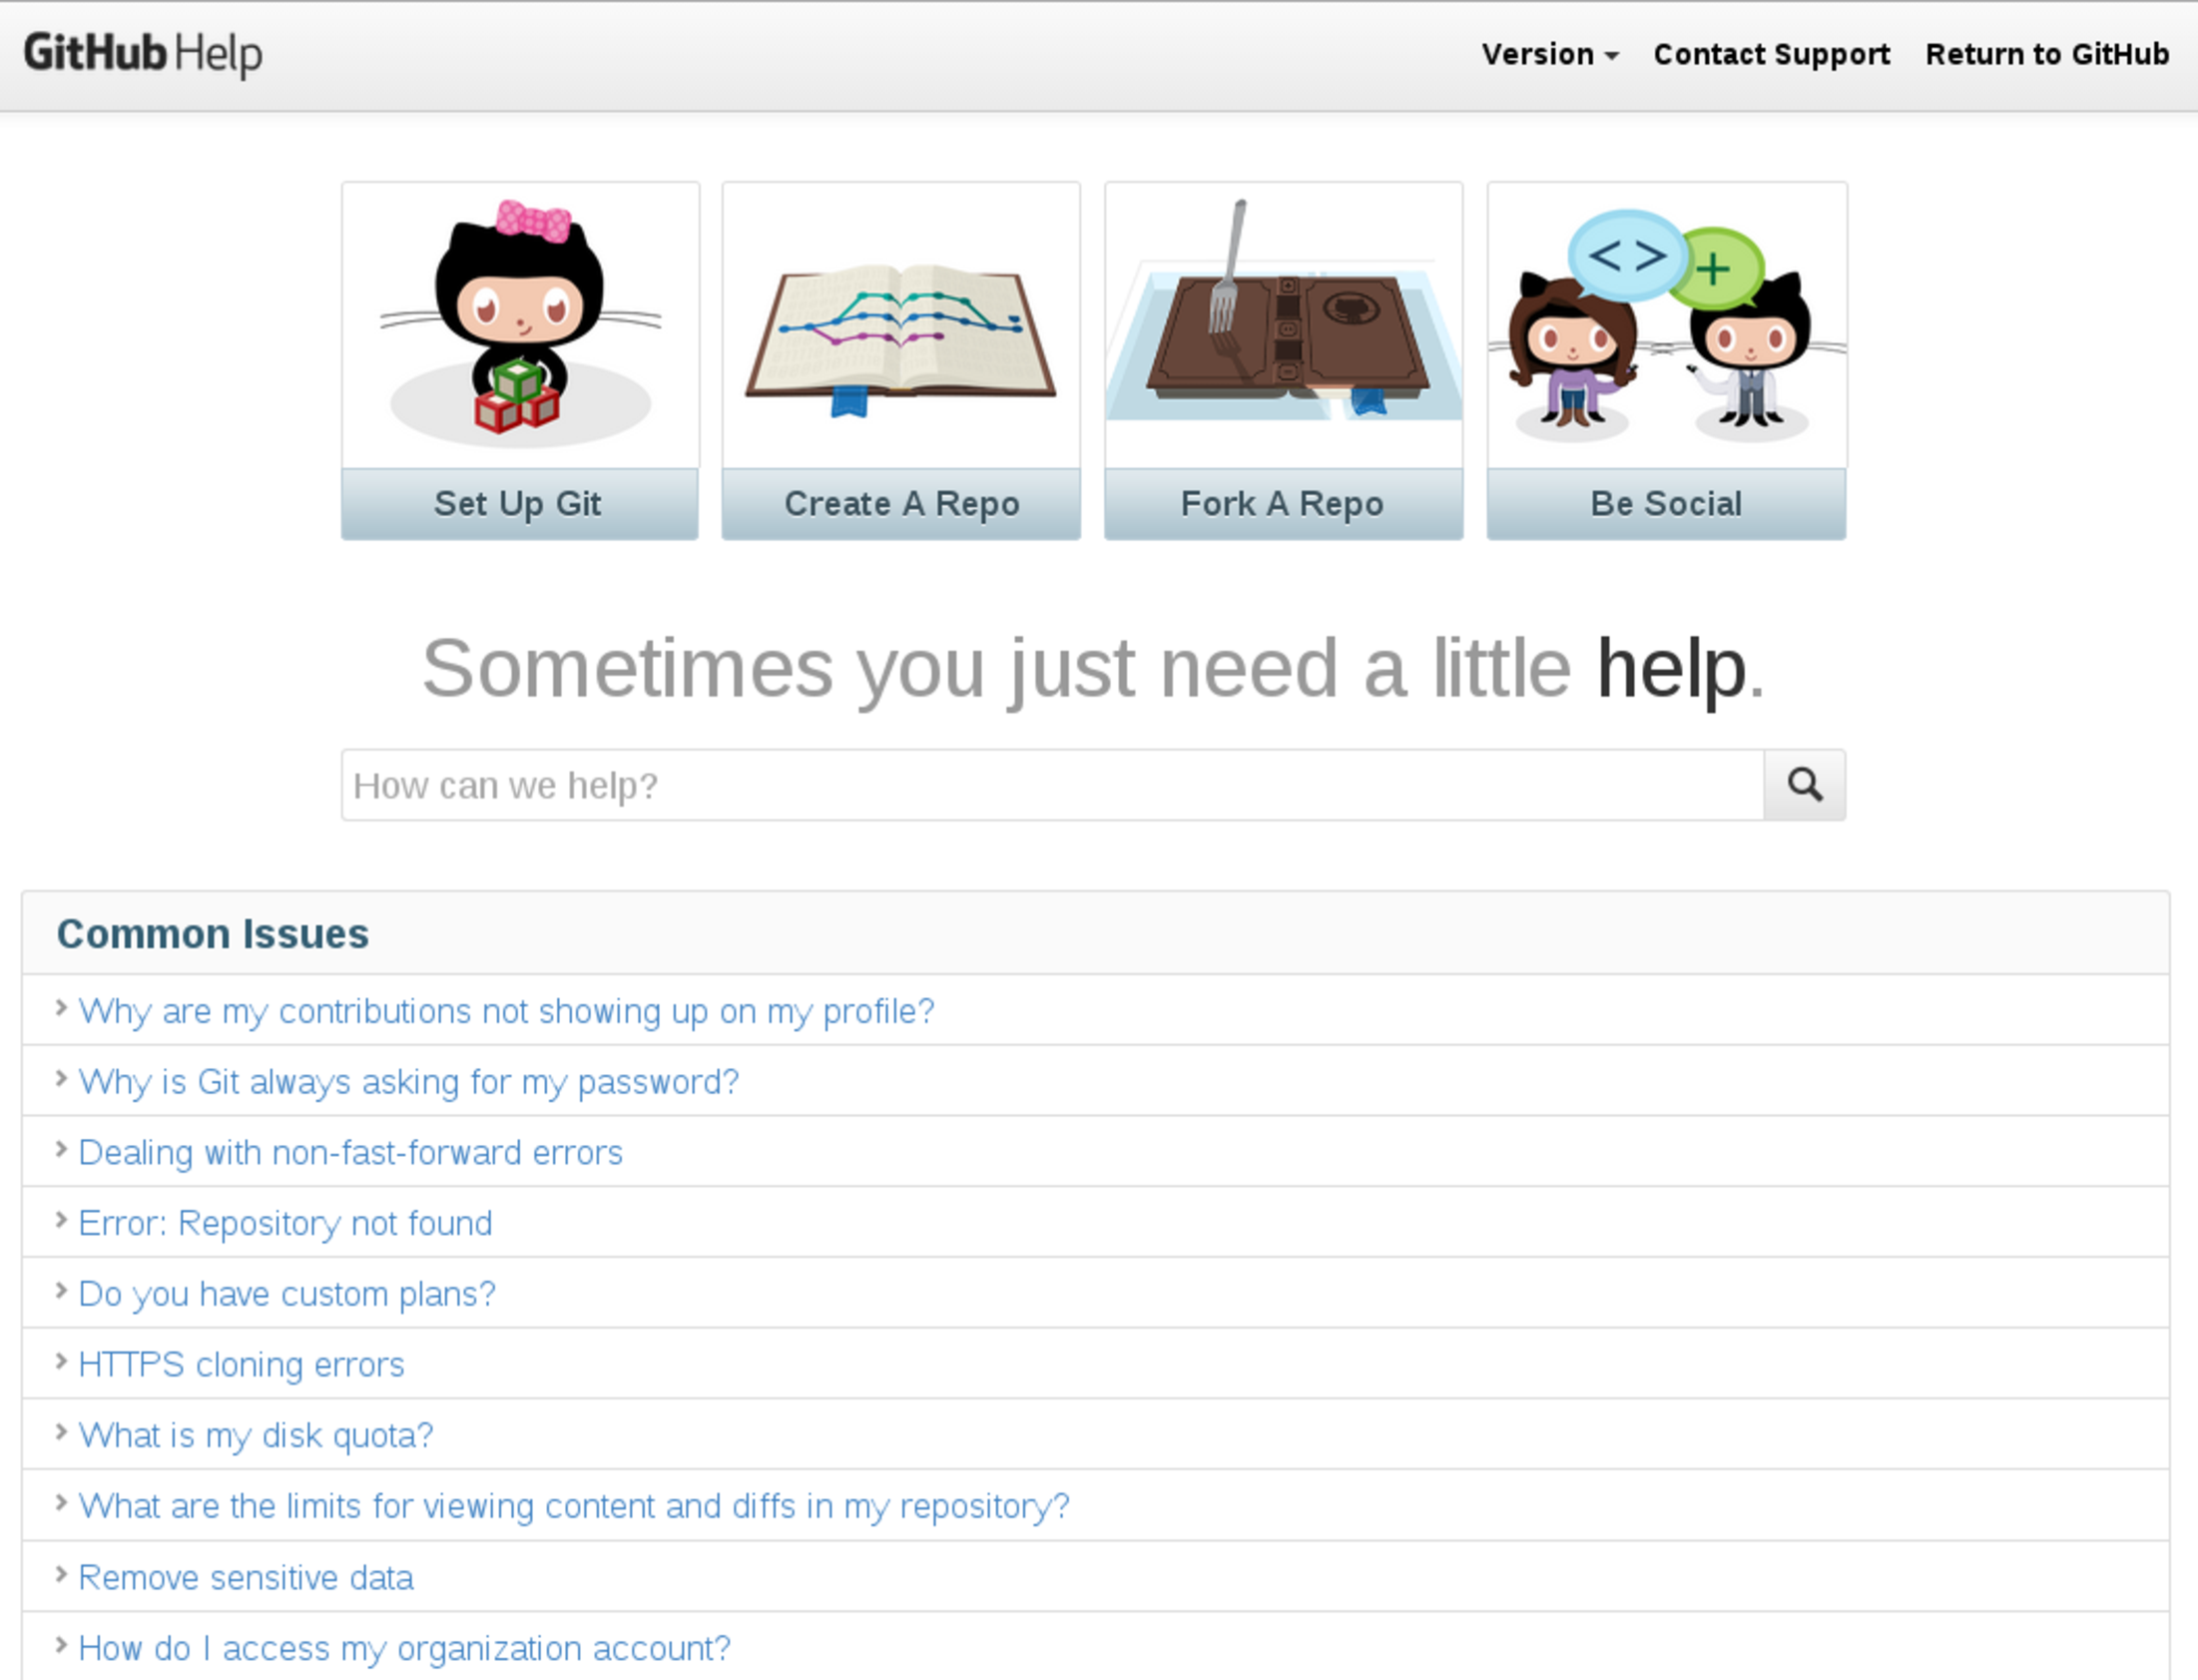
\includegraphics[width = 0.95\textwidth]{/home/ben/Intro_to_R/GitHub_Slides_Source/Images/Git_Resources/GitHub_Help_Page.pdf}
\end{figure}

\end{center}

\end{frame}


\begin{frame}
\frametitle{References}
\bibliographystyle{apalike}
\bibliography{~Intro_to_R/GitHub_Slides_Source/Bib/VC_with_GitHub}
\end{frame}

\begin{frame}
\frametitle{Image Credits}
\begin{itemize}
\item Git Logo by Jason Long \url{http://git-scm.com/downloads/logos}
\item GitHub Logo 
\item R Logo
\end{itemize}
\end{frame}

\end{document}
